% !TEX root = ../Dokumentation.tex
\subsection{Entladen}

\textbf{Funktionsbeschrieb}\\[0.2cm]
\begin{figure}[H]
\centering
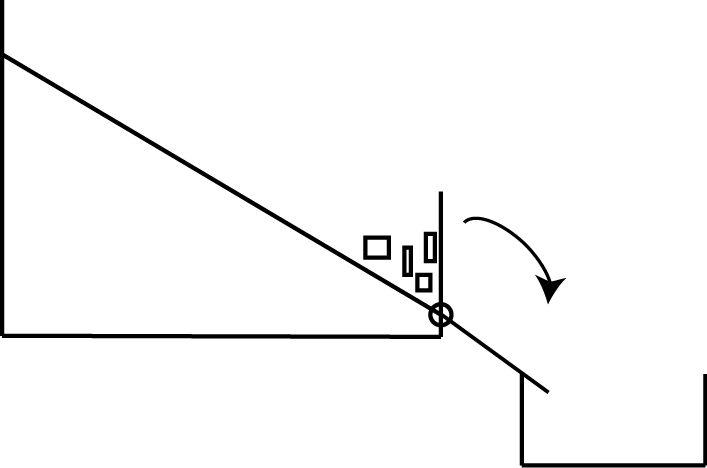
\includegraphics[width=0.5\textwidth]{03_Loesungskonzept/pictures/Entladen_Schraegbehaelter.png}
\caption{Entladen}
\end{figure}

Beim Entladevorgang fährt das Fahrzeug bis auf 20mm +/- 5mm an den Rand des Entsorgungsbecken. Anschliessend wird die Klappe gelöst und diese fällt auf den Rand des Entsorgungsbecken. Über die Klappe rutscht das Schüttgut in das Entsorgungsbecken. Nach erfolgter Abladung fährt das Fahrzeug kurz nach links, damit das ganze Fahrzeug im Zielbereich steht. Dabei hängt die Klappe nach unten.

\textbf{Komponentenbeschrieb}\\[0.2cm]
Die Klappe besteht aus einem handelsüblichen Scharnier auf dem eine Platte aus Acrylglas befestigt ist.
Die Klappe wird von einem gleichen Servomotor wie für den Greifer gehalten.\\
Technische Daten des Motors Entladeklappe:
\begin{itemize}
\item Stellzeit bei 4.8 Volt: 0.1 sec (50°) 
\item Stellzeit bei 6 Volt: 0.08 sec (50°) 
\item Betriebsspannung: 4.6/6 V
\item Stell-Moment bei 4.8 Volt: 18 Ncm
 \item Stell-Moment bei 6 Volt: 20 Ncm 
\end{itemize}

\textbf{Berechnungen}\\[0.2cm]
Die Berechnungen zum Servo Motor für die Klappe sind schon im Kapitel Beladen zu finden.